\documentclass[11pt]{article}

\usepackage{fullpage}
\usepackage{caption}
\usepackage{float}

\usepackage[T1]{fontenc}
\usepackage{textcomp}

\usepackage[english]{babel}
\usepackage[utf8]{inputenc}

\usepackage{lmodern}

\usepackage{hyperref}
\hypersetup{breaklinks}
\hypersetup{pdfborder=0 0 0}

\usepackage[babel=true]{microtype}


\usepackage{amsmath}
\renewcommand{\vec}[1]{\mathbf{#1}}
\newcommand{\mat}[1]{\mathbf{#1}}
\DeclareMathOperator{\Prob}{Prob}
\newcommand{\md}{\mathrm{d}}
\newcommand{\me}{\mathrm{e}}
\newcommand{\mT}{\mathrm{T}}

\usepackage{units}
\usepackage{tikz}
\usepackage[square,sort,comma,numbers]{natbib}
\usepackage{hypernat}

\allowdisplaybreaks[1]

\title{Supporting Information: \\
\textbf{Interactions between chronic diseases: asymmetric outcomes of co-infection at individual and population scales}}
\date{}
\author{Erin E. Gorsich$^{a,b*}$, Rampal S. Etienne$^{c}$, Jan Medlock$^{a}$, \\ Brianna R. Beechler$^{a}$, Johannie M. Spaan$^{b}$, Robert S. Spaan$^{d}$, \\Vanessa O. Ezenwa$^{e}$, Anna E. Jolles$^{a,b}$}

\begin{document}

\maketitle

\noindent{}a. Department of Biomedical Sciences, 105 Dryden Hall, Oregon State University \\
\noindent{}b. Department of Integrative Biology, Cordley Hall, Oregon State University \\
\noindent{}c. Groningen Institute for Evolutionary Life Sciences, University of Groningen, The Netherlands\\
\noindent{}d. Department of Fisheries and Wildlife, 104 Nash Hall, Oregon State University \\
\noindent{}e. Odum School of Ecology and Department of Infectious Diseases, College of Veterinary Medicine, University of Georgia \\
\noindent{}$ \ast$ Corresponding author e-mail: eringorsich@gmail.com \\



\noindent \Large{\textbf{Appendix 1. Additional information on statistical analyses}}\\
%\normalize

{\subsection*{Mortality}}
Our mortality dataset included 127 individuals and 38 mortality events. We estimated the time of mortality as midway between the last capture period the animal was observed and the subsequent capture period (6 months later) when it was recovered unless the exact mortality date was known. This assumption is supported by
our sampling design that recovered most animals quickly after death. For 20 of the mortality events included here, we were able to estimate the mortality date within one month of error by comparing the date the animal was last observed with the date it was known to be dead. Animals were identified as dead by either finding the carcass or recovering the radio-collar. All radio-collars were recovered before the subsequent capture period. The high recapture rates in this study made the Cox proportional hazards model an acceptable representation of the time-to-event process \cite{fisher_time-dependent_1999}. We evaluated the proportional hazards assumption of the model using Schoenfeld residuals \cite{grambsch_proportional_1994, fox_cox_2011} quantified with the cox.zph function in the survival package \cite{therneau_package_2014}.
To test for differences in the distribution of mortality times in uninfected and infected buffalo, we included the presence or absence of brucellosis-positive test result ($bruc_i$) and a BTB-positive test result ($BTB_i$) as time-dependent explanatory variables. We also account for the buffalo's age at first capture ($agecat_i$) and capture location ($site_i$) as time-independent, categorical variables. These main effects and interaction terms give the following full model:
\begin{gather*}
h_{i}(t) \sim h_{0}(t) \text{exp} (\beta_{1} BTB_i + \beta_{2} bruc_i + \beta_{3,j}agecat_i + \beta_4 site_i + \\
\beta_5 BTB_i * bruc_i + \beta_{6,j} BTB_i * agecat_i + \beta_{7,j} bruc_i * agecat_i + \\
 \beta_8 BTB_i * site_i + \beta_9 bruc_i * site_i)
\end{gather*}

where $h_{i}(t)$ represents the hazard function for the i th individual and describes the instantaneous risk of mortality at time, t, conditional on survival to that time. The baseline hazard is represented by $h_{o}(t)$ and remains unspecified.  

We conducted model selection in two stages. First, we considered the relationship between the buffalo's age at first capture and mortality rate by only considering age as a predictor of mortality. This is because both infections are assumed to be life-long, so we were concerned that the positive association between age and testing positive for both infections could bias our results. We considered 4 potential representations of age as an explanatory variable (age1: late development with a sub-adult category, 1-2.9, 3-5.9, 6+; age2: late development without a sub-adult category, 1-2.9, 3+; age3: early development with a sub-adult category, 1-1.9, 2-4.9, 5+; age4: early development without a sub-adult category, 1-1.9, 2+). The age categories representing late development (age1: 1-2.9, 3-5.9, 6+, age2: 1-2.9, 3+) provided better fits based on AIC (Akaike information criterion) compared to the age categories representing early development with the same number of parameters (age3: 1-1.9, 2-4.9, 5+, age4: 1-1.9, 2+). The addition of an extra age category had a minimal effect on model fit. The AIC values for each model were, 330.9, 329.9, 336.6, and 335.8, for models including age1, age2, age3, and age4, respectively. Second, we conducted a formal model selection following the full model in equation 1 with age2 representing the covariate for age. We used backwards selection by sequentially removing interaction terms and then main effects terms based on drop-in-deviance $\chi^2$ tests. From the final model, we evaluate $\beta_1$ to determine the mortality consequences of BTB, $\beta_2$ to determine the mortality consequences of brucellosis, and $\beta_5$ to determine if buffalo co-infected with both pathogens have exacerbated mortality.

We converted these parameters into infection-specific mortality rates by interpreting the exponentiated model coefficients as having a multiplicative effect on the mortality hazard (e.g. the mortality rate in buffalo with BTB is equal to the mortality rate in susceptible buffalo multiplied by exp($\beta_1$)). 
\begin{table}[H]
\centering
\caption*{\textbf{Table S1.} Parameter values ($\beta$), standard errors (SE), and significance tests (Z-value, p-values) for each covariate in the final model. A positive parameter value for BTB or brucellosis indicates an increased mortality hazard by a factor of exp($\beta$). A positive parameter for site indicates higher mortality in the Crocodile Bridge capture site compared to Lower Sabie. A positive parameter for age indicates higher mortality in juveniles (age $<3$) compared to adults (age $\geq 3$).  The data contained 127 animals and 38 mortality events.}
\newcommand{\head}[1]{\textnormal{\textbf{#1}}}
\normalsize
\begin{tabular}{lcccc} 
\hline
\head{Parameter     } & \head{     Estimate ($\beta$)     } & \head{     SE     } & \head{     Z-value     } & \head{     p-value     } \\*
\hline
BTB ($\beta_1$) & 1.04 & 0.35 & 2.98 & 0.003 \\
bruc ($\beta_2$)  & 1.11 & 0.35 & 3.16 & 0.002\\
age ($\beta_3$) & 1.18 & 0.33 & 3.35 & < 0.001\\
site ($\beta_4$) & 0.74 & 0.32 & 2.27 & 0.023\\
\hline 
\end{tabular}
\end{table} 
 
\pagebreak 

\subsection*{Fecundity}
We assessed the effects of infection and co-infection on fecundity by testing for an association between infection status and reproductive status, defined as having a calf. Birthing in African buffalo occurs seasonally, with most births occurring from December to March (5). Buffalo calves are often weaned approximately 5-6 months later \cite{winthrop_bovine_1988}. 
We, therefore, expected calf observations to be less accurate just before or during birthing season and account for this by only including captures immediately following the birthing season (March to July). Calving is strongly age-dependent and only buffalo 4 years of age or older were considered in this analysis, following previous analyses of buffalo fecundity \cite{gorsich_context-dependent_2015}. 
The resulting dataset includes 143 observations from 62 buffalo over the course of our longitudinal study. 
Of the 143 observations, 29\% were observed with a calf at heel. 
Uninfected adult buffalo (age $\geq$ 5) were observed with a calf at heel 68\% (11/16) of the time, buffalo with BTB were observed with a calf at heel 37\% (6/16) of the time, buffalo with brucellosis were observed with a calf at heel 29\% (7/24) of the time, and co-infected adults were observed with a calf at heel 57\% (4/7) of the time.


We tested if reproductive status is associated with infection status with a generalized linear mixed model with binomial errors and a logit link function for the response.  
We considered all main effects and interactions specified for previous analyses as dependent variables: BTB infection, brucellosis infection, age, capture site and interactions between BTB-brucellosis, BTB-age, BTB-site, brucellosis-age, and brucellosis-site. 
Animals were sampled over time, so we accounted for animal ID as a random effect.

We conducted model selection on the fixed effects in two stages.
First, we considered the relationship between the buffalo's age and fecundity by only considering age as a predictor. 
In this analysis, the age categories representing early development (age3 = 1-1.9, 2-4.9, 5+, AIC = 166.5) provided better fits compared to age categories representing late development (age1 = 1-2.9, 3-5.9, 6+, AIC = 168.5). 
Second, we conducted a formal model selection following the full model with age3 representing the covariate for age. 
Model selection was conducted by sequentially removing interaction terms and then main effects terms based on drop-in-deviance $\chi^2$ tests.
After model selection, only age was a significant predictor of fecundity (Z = 3.30, p-value = 0.001).  The odds of a buffalo being observed with a calf were 3.84- fold (95\% CI 1.73- 8.54) higher in adult buffalo aged over 5 years old compared to sub-adult buffalo aged less than 5 years.


\begin{figure}[H]
\centering
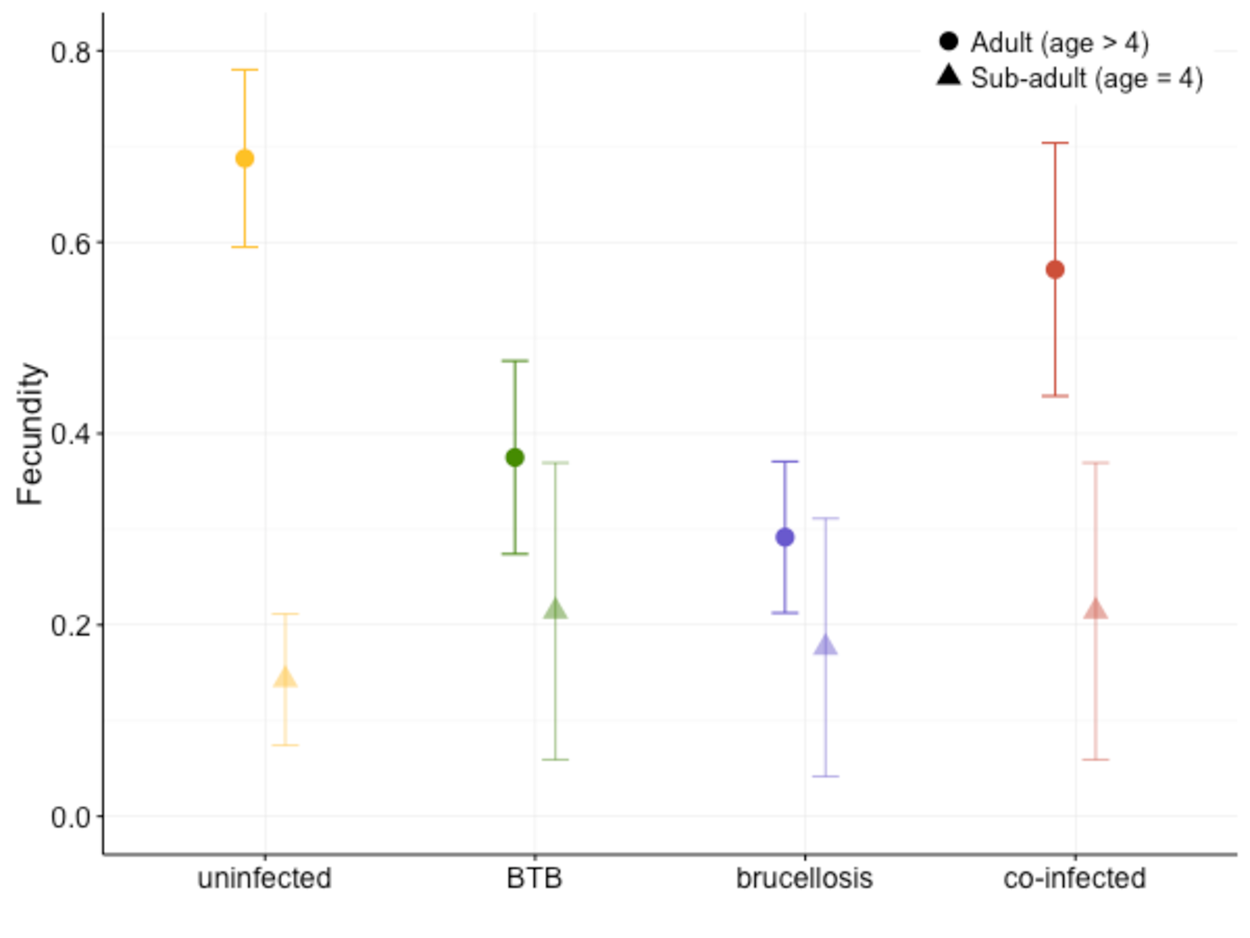
\includegraphics[width=.99\linewidth]{Figure_S1.pdf}
\caption*{\textbf{Fig S1.} Proportion of buffalo observed with a calf.  Proportion estimates and standard errors are based on the number of observations with a calf in the data.}
%\label{fig:figS1}
\end{figure}

\pagebreak

\subsection*{Infection risk}
Our dataset for brucellosis incidence included 26 brucellosis incidence events in the 110 buffalo who were sero-negative at their first capture (Fig S2). Our dataset for BTB incidence included 36 BTB incidence events in 131 buffalo. We used Cox proportional hazards models to test for differences in the distribution of infection times in uninfected buffalo and buffalo that tested positive for the second infection. Using the same co-variates and model selection procedure described in Table S1, we fit the following full model,

\begin{gather*}
h_{i}(t) \sim h_{0}(t) \text{exp} (\beta_{1} infection_i + \beta_{2,j} agecat_i + \beta_3 site_i \\
+ \beta_{4,j} infection_i agecat_i + \beta_{5} infection_i site_i 
\end{gather*}

where $h_{i}(t)$ represents the hazard function for the $i^{th}$ individual and describes the instantaneous risk of infection at time, t, conditional on the individual not becoming infected until that time. For models predicting brucellosis infection risk, we evaluate $\beta_1$ to estimate the consequences of BTB infection on brucellosis infection risk, $\beta_4$ to determine if the consequences of BTB vary across age groups, and $\beta_5$ to determine if the consequences of BTB vary between sites. Similarly, for models predicting BTB infection risk, we evaluate $\beta_1$ to estimate the consequences of brucellosis infection on BTB infection risk, $\beta_4$ to determine if the consequences of brucellosis vary across age groups, and $\beta_5$ to determine if the consequences of brucellosis vary between sites.

For both infections, the age categories representing late development (age1 = 1-2.9, 3-5.9, 6+, age2 = 1-2.9, 3+) provided better fits compared to the age categories representing early development with the same number of parameters (age3 = 1-1.9, 2-4.9, 5+, age4 = 1-1.9, 2+). However, we were unable to consider age1 as a co-variate because none of the 8 buffalo aged 6 years or older at the initial capture became infected with brucellosis.  AIC values for were 248.03, 250.04, and 251.63 for models predicting brucellosis infection with age2, age3, and age4 included as a predictor, respectively. AIC values were 347.80, 349.37, and 349.26 for models predicting BTB infection with age2, age3 and age4 included as a predictor. Thus, we conducted a formal model selection for brucellosis and BTB incidence following the full model with age2 representing the covariate for age. 

 We note that the effect of BTB infection on brucellosis incidence varied by capture site ($\beta_5$, BTB:site). Buffalo infected with BTB were associated with a 4.32 (95\%CI 1.51-12.37) times higher rate of brucellosis infection at the Lower Sabie site while buffalo infected with BTB at the Crocodile Bridge site had similar incidence rates compared uninfected buffalo (Z = - 0.821, p-value = 0.412). The parameters for our disease model are based on the effect of BTB taken across both sites: buffalo infected with BTB faced a 2.09 (95\% CI 0.89-4.91) fold higher risk of acquiring brucellosis (Z = 1.742, p-value = 0.081).

\begin{table}[H]
\centering
\caption*{\textbf{Table S2.} Parameter values, standard errors, and significance tests (Z-value, p-values) are shown for each covariate in the final model. A positive parameter value for BTB or brucellosis indicates an increased mortality hazard by a factor of exp$(\beta)$. A positive parameter for site indicates higher infection risk in Crocodile Bridge capture site compared to Lower Sabie. A positive parameter for age indicates a higher infection risk in juveniles (age <3) compared to adults (age $\geq$ 3). }
\newcommand{\head}[1]{\textnormal{\textbf{#1}}}
\normalsize
\begin{tabular}{lcccc} 
\hline
\head{Parameter     } & \head{     Estimate ($\beta$)     } & \head{     SE     } & \head{     Z-value     } & \head{     p-value     } \\*
\hline
\textbf{Brucellosis incidence} & & & & \\
BTB ($\beta_1$) & 1.46 & 0.54 & 2.73 & 0.006 \\
age ($\beta_2$) & 1.89 & 0.43 & 2.06 & 0.039\\
site ($\beta_3$) & 0.71 & 0.51 & 1.41 & 0.158 \\
BTB:site ($\beta_5$) & -2.40 & 1.20 & -2.01 & 0.045 \\
 & & & & \\
\textbf{BTB incidence}  & & & & \\
age ($\beta_2$) & -0.61 & 0.37 & -1.65 & 0.10 \\
site ($\beta_3$) & -0.70 & 0.35 & -2.02 & 0.04\\
\hline 
\end{tabular}
\end{table} 


\begin{figure}[H]
\centering
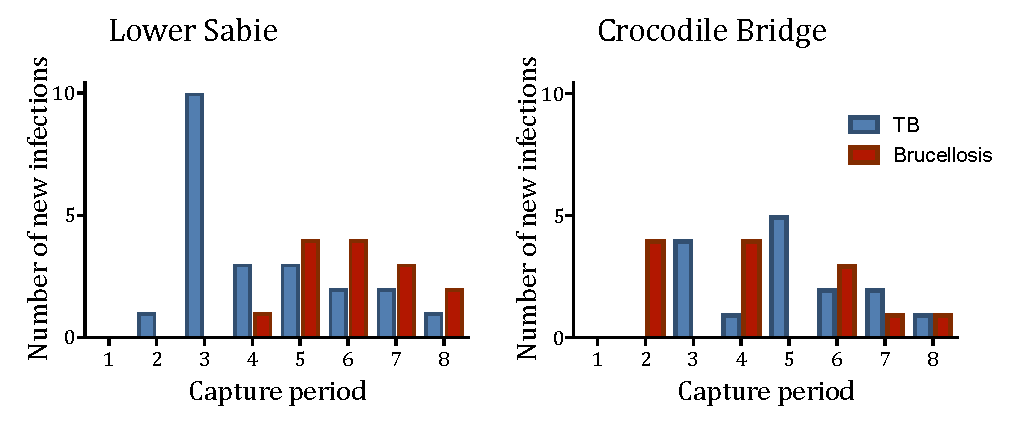
\includegraphics[width=.99\linewidth]{Figure_S2.pdf}
\caption*{\textbf{Fig S2.} The number of new BTB and brucellosis infections over the course of the study in buffalo initially captured in the Lower Sabie and Crocodile Bridge sites show that infections occurred continuously over the study period.}
%\label{fig:figS1}
\end{figure}




\pagebreak

\bibliographystyle{pnas-new}
\bibliography{coinfection}




\end{document}